\documentclass[a4paper, twoside, 11pt]{article}

% === Useful packages ===
\usepackage[german]{babel}
\usepackage[margin=2cm]{geometry}
% \usepackage[top=2cm,bottom=2cm,left=2cm,right=2cm]{geometry}

% text
\usepackage{amsthm, amsmath, amssymb}
\tolerance=1
\emergencystretch=\maxdimen
\hyphenpenalty=10000
\hbadness=10000
\parindent=0pt % remove indentation after figures
\usepackage{setspace} 
\onehalfspacing 
\raggedbottom % removes space between paragrafs
\linespread{1.15}
\usepackage{xcolor}

% --- manage images ---
\usepackage{graphicx} %\includegraphics[width=\textwidth]{path.png}
\graphicspath{ {img/} }
\usepackage{float}

% --- manage multicols ---
\usepackage{multicol}
\usepackage{paracol}
\setcolumnwidth{0.30\textwidth}
\setlength\columnsep{20pt}
\setlength{\columnseprule}{0.5pt}

\title{Regelungstechnik  \\ [1ex] \large Fachsemester 3}
\author{Prof. Dr.-Ing. habil. Klaus-Peter Döge}
\date{}

\begin{document}
\maketitle


\newpage
 \section*{\centering 15.10.2024}

  x) Regelgröße:
  - die physikalische Größe, die geregelt werden soll. Das bedeutet ein physikalischer Wert in einem gewünschten Maß gehalten wird.

  w) Führungsgröße:
  -

  y) Stellgröße:
  - physikalische Größe, welche die Regelgröße auf eine gewünschte Weise beeinflusst. (Bsp. Volumen Strom)

  e) Regelabweichung:
  - Differenz = Führungsgröße - Regelgröße

  z) Störgröße:
  - Einflüsse die selbst nicht beeinflusst werden können
  - Größen, die eine eingestellte Regelung aus dem Gleichgewicht bringt.

  Regelstrecke:
  - ist das zugrunde liegende System

  Systemarten: (Eingang/Ursache - Ausgang/Wirkung)
  - Intigrator: bsp. Volumenstrom wird in Volumen aufintigriert
  - Verstärker: bsp. Hebel


\newpage
\section*{\centering 17.10.2024 (Semesteranfang muss noch nachgetragen werden)}
\section*{\centering 22.10.2024 (Semesteranfang muss noch nachgetragen werden)}
\section*{\centering 24.10.2024 (Semesteranfang muss noch nachgetragen werden)}
\section*{\centering 29.10.2024 (Semesteranfang muss noch nachgetragen werden)}
\section*{\centering 05.11.2024 (Semesteranfang muss noch nachgetragen werden)}
\section*{\centering 07.11.2024 (Semesteranfang muss noch nachgetragen werden)}


\newpage
\section*{\centering 12.11.2024 (muss wegen Krankheit noch nachgetragen werden)}
\section*{\centering 14.11.2024 (muss wegen Krankheit noch nachgetragen werden)}

\newpage
\section*{\centering 19.11.2024}
\subsection*{Wiederholung}
\subsubsection*{Merken:}
\begin{itemize}
	\item Impulsfunktion $\delta (t)$ $\rightarrow$ Gewichtsfunktion $g(t)$
	\item Sprungfunktion $\alpha (t) _{falsche variable kann aber in den Folien nachgeschaut werden}$ $\rightarrow$ Übergangsfunktion $h(t)$
	\item (für die Rücktransformation sollte Partialbruchzerlegung sitzten)
\end{itemize}

\subsubsection*{Operationsverstärker}
(siehe Folien)

\subsubsection*{Bode-Diagram}
(siehe Folien) $\rightarrow$ Selbststudium

\subsubsection*{Übergangs- und Gewichtfunkiton}
(siehe Folien) $\rightarrow$ Selbststudium

\subsubsection*{Übergangs- und Gewichtfunkiton}
(siehe Folien) $\rightarrow$ Selbststudium

\newpage
\subsection*{Teil 2 - Der Regler}
\subsubsection*{Der PID-Regler: der linearer Regler}
PID $\rightarrow$ besteht aus den drei basis Übertragungsgliedern \\
Warum PID und nicht PT1 etc.?: PT1/ PT2 sind langsamer als der P-Anteil des PID \\

Nomenklatur lernen: 
\begin{itemize}
	\item Sprungantwort $\rightarrow$ Übergangsfunktion
	\item Eingangssignal $x_e(t)$ $\rightarrow$ Regel-Abweichung
	\item Ausgangssignal $x_a(t)$ $\rightarrow$ Stellgröße
\end{itemize}

\[
G(s) = V(1+ \frac{1}{sT_N}+ sT_V)
\]
V = Verstärkung
\begin{multicols}{3}
	P-Anteil: lorem $\rightarrow$  1

	\columnbreak
	I-Anteil: Intigration $\rightarrow$ $\frac{1}{sT_N}$

	\columnbreak
	D-Anteil: Differentation $\rightarrow$ $sT_V$ \\
	(Sprungänderung ist im Einschaltmoment unendlich)
\end{multicols}
\begin{center}
	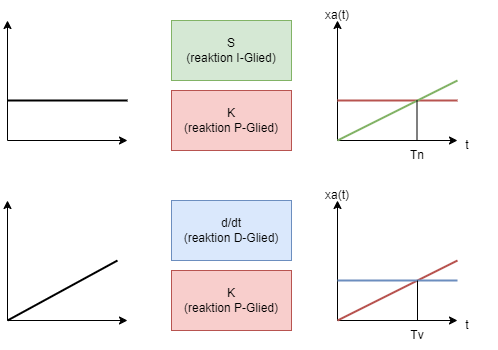
\includegraphics[width=0.6\textwidth]{19_11_2024_reglungstechnik.png}
	% 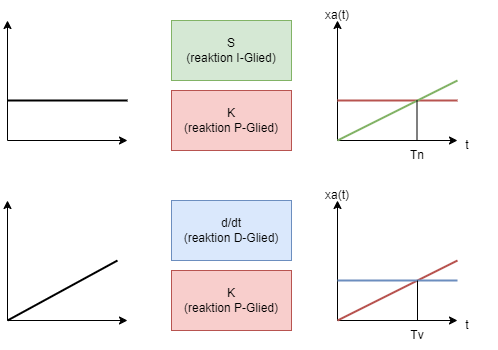
\includegraphics[width=0.5\textwidth]{19_11_2024_reglungstechnik.png}
\end{center}

Typische Anwendung der Glieder: 
\begin{multicols}{3}
	P-Regler nehmen \\
	weil?

	\columnbreak
	PI-Regler \\
	falls P nicht möglich \\
	weil?

	\columnbreak
	PID-Regler \\
	falls PI nicht möglich \\
	weil?
\end{multicols}


\newpage
\section*{\centering 21.11.2024}
\subsection*{Standardregelkreis}
Regelkreis nach DIN 19226 \\
(Grafik im Script zu finden und bereits angefangen)

\subsection*{Führungs und Störverhalten (Thema 11)}
Führungsverhalten: Wie reagiert der Regelkreis auf eine Änderung der Führungsgröße (w(t))? \\
Störverhalten: Wie reagiert der Regelkreis auf eine Änderung der Störgröße (z(t))? \\
(Grafik im Script zu finden und bereits nachgebastelt)

\subsubsection*{Berechnung der Regelgröße in Abhängigkeit der Führungsgröße}
$w(s) \rightarrow x(s)$
\[ X(s)=(W(s)-X(s)) * G_0(s) \]
$G_0(s)=\frac{X(s)}{E(s)} = \frac{X(s)}{W(s)-X(s)}$
\[ X_W(s)=\frac{G_0(s)}{1+G_0(s)} * W(s) \]
\[ G_{WX}(s)=\frac{X(s)}{W(s)} = \frac{G_0(s)}{1+G_0(s)} \]

\subsubsection*{Berechnung der Regelgröße in Abhängigkeit der Führungsgröße}
$w(s) \rightarrow \epsilon(s)$ (oder auch E(s))
\[ E(s)=W(s)-X(s); X(s)=E(s)*G_0(s) \]
\[ E(s)=W(s)-(E(s)*G_0(s)) \]
\[ E_W(s)=\frac{1}{1+G_0(s)}*W(s) \]
\[ G_{WE}(s)=\frac{E(s)}{W(s)}=\frac{1}{1+G_0(s)} \]

\subsubsection*{Berechnung der Regelgröße in Abhängigkeit der Störgröße}
$z(s) \rightarrow x(s)$
\[ X(s)=-X(s)*G_0(s)+Z(s) \]
\[ X_Z(s)=\frac{1}{1+G_0(s)}*Z(s) \]
\[ G_{ZX}(s)=\frac{X_Z(s)}{Z(s)}=\frac{1}{1+G_0(s)} \]

\subsubsection*{Berechnung der Regelabweichung in Abhängigkeit der Störgröße}
$z(s) \rightarrow \epsilon(s)$ (oder auch E(s))
\[ E(s)=-X(s); X(s) = E(s) * G_0(s)+Z(s) \]
\[ E(s)=-(E(s)*G_0(s)+Z(s)) \]
\[ E_Z(s)=-\frac{1}{1+G_0(s)}*Z(s) \]
\[ G_{ZE}(s)=\frac{E_Z(s)}{Z(s)}=-\frac{1}{1+G_0(s)} \]

\subsubsection*{Kombination von Störungs- und Führungsverhalten}
Führ die Formelsamlung: (Graftk/Zusammenfassung im Script zu finden) \\
Addition/Überlagerung von Signalen dürfen in linearen Systemen vollzogen werden.


\subsection*{Einstellregel (Thema 15)}
Wie stellt man einen Reglner ein? \\
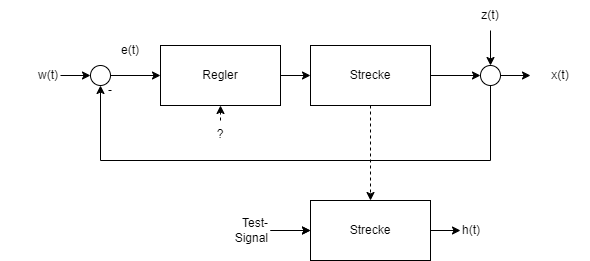
\includegraphics[width=\textwidth]{2024_11_21_Wie_stelle_ich_einen_Regler_ein.png}
(weitere Grafik im Script)\\
\begin{itemize}
	\item $T_U$ ist eine Erstatz tot-Zeit
	\item $T_G$ ist eine Ersatz-Zeit-Konstante
\end{itemize}
Zwei Varianten weil eine Regelstrecke mit I-Anteil (ohne Ausgleich) ist nicht begrentzt \\
(rest ist im Script zu finden)


\newpage
\section*{\centering 26.11.2024}
\subsection*{Regelabweichung (Thema 12)}
(für weitere Grafiken oder Unklarheiten durch fehlende Grafiken bitte in das Script der Vorlesung schauen) \\
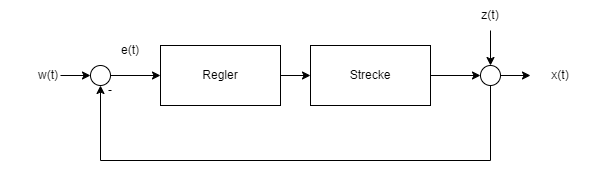
\includegraphics[width=\textwidth]{2024_11_26_standard_regelkreis.png}
($W(s) = \frac{W_0}{s}$) \\
Der Standardregelkreis fasst kein Messglied. (Es wird trotzdem gemessen. Es wird nur nicht abgebildet) \\
\begin{multicols}{2}
	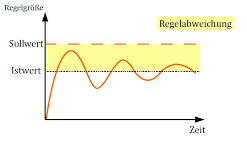
\includegraphics{2024_11_26_regelabweichung.png}

	\columnbreak
	
	\begin{center} $e = w - x$ \end{center}
	Die Berechnung der Regelabweichung erfolgt im stationären Zustand. $\to $ Bleibende Regelabweichung
\end{multicols}
\vspace{1em}
(Berechnung des Vorlesungs / Script Bsp.)
\begin{itemize}
	\item P-Regler
	\begin{center}
	$\lim_{t \to \infty} e(t) = \lim_{s \to 0} E(s) \cdot \textcolor{red}{s}$ \\ \mbox{} \\
	$E_w(s) = \frac{1}{1+G_0(s)} \cdot W(s)$ mit $G_0(s) = G_R(S) \cdot G_S(s)$; $G_R(s) = K$ \\ \mbox{} \\
	$E_W(s) = \frac{1}{1+a \cdot K} \cdot \frac{W_0}{s}$ \\ \mbox{} \\
	$\lim_{t \to \infty} e(t) = \lim_{s \to 0} \frac{1}{1+a \cdot K} * \frac{W_0}{s} \cdot \textcolor{red}{s} = \frac{W_0}{1+a \cdot K}$
	\end{center}
	a - Verstärkung des Öldruckpresse\\
	(Vorlesungs/Script Bsp. würde vermutlich ein I-Anteil beinhalten, um mehr Genauigkeit zu erhalten.)

	\item I-Regler
	\begin{center}
	$G_R(s) = \frac{1}{sT_N}$ \\ \mbox{} \\
	$E_W(s) = \frac{1}{1+G_0(s)} \cdot W(s) = \frac{1}{1+a \cdot \frac{1}{T_Ns}} \cdot \frac{W_0}{s}$ \\ \mbox{} \\
	$\lim_{t \to \infty} e(t) = \lim_{s \to 0} \frac{1}{1+a \cdot \frac{1}{T_Ns}} \cdot \frac{W_0}{s} \cdot \textcolor{red}{s}$ \\ \mbox{} \\
	$\lim_{s \to 0} \frac{1 W_0}{1 + \frac{a}{T_Ns}} = 0$ \\ \mbox{} \\
	$\lim_{s \to 0} \frac{s \cdot W_0}{s + \frac{a}{T_N}} = 0$
	\end{center}
	(I-Regler ist für die meisten Fälle zu langsam)
	
	\item PI-Regler \\
	Dieser Regler ist schnell und genau genug.
\end{itemize}

\paragraph{Ein weiters Beispiel für das Selbststudium (im Script)} \mbox{} \\
PT2-Glied $\to$ Nicht Schwinungsfähig
\begin{center}
	$E(s) = W(s) - [uebertragungsfunktionen] E(s)$
\end{center}


\newpage
\section*{\centering 03.12.2024}
\subsection*{Das Nyquist-Verfahren (Thema 14)}
\vspace{1em}
\columnratio{0.5}
\begin{paracol}{2}
	\underline{Hurwitz} \\
	Prüfung: an geschlossener Kette
	\switchcolumn
	\underline{Nyquist} \\
	Prüfung: an offener Kette \\
	Vorteil: Experimentelle Herangehensweise
\end{paracol}
\paragraph{Erklärung} \mbox{} \\
\begin{figure}[ht]
	\centering
	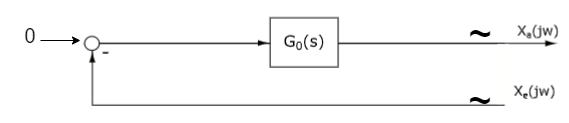
\includegraphics[width=0.8\textwidth]{2024_12_03_nyquist.png}
	\caption{Offene Regelkette}
\end{figure}
\[ G_0(j\omega) = \frac{X_a(j\omega)}{X_e(j\omega)} = -1 \]

\vspace{1em}

Der geschlossene Regelkreis ist stabil, wenn die ortskurve des Frequenzgangs der offenen Kette den kritischen Punkt nicht umschließt. Bzw. links davon sind.
\begin{figure}[ht]
	\centering
	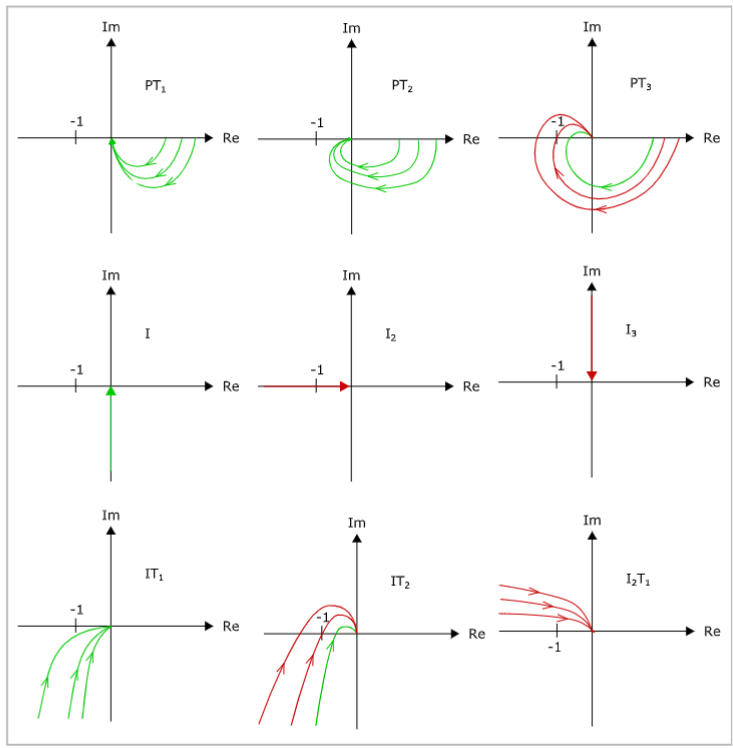
\includegraphics[width=0.6\textwidth]{2024_12_03_nyquist_ortskurven.png}
	\caption{Niquist Ortskurven}
\end{figure}

Randnotiz: $I_1$-Glied $=\frac{1}{s} = \frac{1}{j\omega}$ \\
Hausaufgabe: Berechnen sie die Übertragungsfunktion einer Rückgekoppelten I-Gliedes

\vspace{1em}
\begin{center}
	\[ G_0(s) = G_R(s) \cdot G_S(s) = \frac{1}{sT_N (1+2s) (1+4s)} \]
	$ s = \delta + j\omega$, $ \delta = 0 $
	\[ G_0(j\omega) = \frac{1}{j\omega T_N (1+2j\omega)(1+4j\omega)} = \frac{-j\omega T_N (1-2j\omega)(1-4j\omega)}{-j\omega T_N (1-2j\omega)(1-4j\omega)} \]
	Zähler $\to$ ausmultipliziert; Nenner $\to$ 3. Binomische Formel
	\[ G_0(j\omega) = \frac{-6\omega^2}{\omega^2 T_N (1+4\omega^2)(1+16\omega^2)} + j \frac{-\omega + 8\omega^3}{\omega^2 T_N (1+4\omega^2)(1+16\omega^2)} \]
	\[ G_0(j\omega) = \frac{-6}{T_N (1+4\omega^2)(1+16\omega^2)} + j \frac{8\omega^2 -1}{\omega T_N (1+4\omega^2)(1+16\omega^2)} \]
	\[ G_0(j\omega) = -1 + 0\]
\end{center}

\paragraph{Grafische Variante des Niquist-Kriterikums} \mbox{} \\
\begin{table}[h]
	\centering
	\begin{tabular}{|c||c|c|c|c|}
	\hline
	$\omega$ 				& Re / $T_N=2$		& Re / $T_N = \frac{4}{3}$ 	& Re / $T_N = 1$	& Im 		\\ \hline\hline
	0						& $-3$ 				& $-4.5$					& $-6$				& $-\infty$ \\ \hline
	$\sqrt{\frac{1}{8}}$ 	& $-\frac{2}{3}$ 	& $-1$ 						& $-\frac{4}{3}$	& 0			\\ \hline
	$\infty$ 				& 0					& 0							& 0					& 0			\\ \hline
							& stabil			& instabil					& instabil			&			\\ \hline
	\end{tabular}
	\caption{Grafik Fehlt}
\end{table}

\paragraph{Analytische Variante des Niquist-Kriterikums}
\begin{enumerate}
	\item $Im\{ G_0(j\omega)\} = 0$ \\
	$8 \omega^2-1=0$; $\omega_{kritisch} = \pm \sqrt{\frac{1}{8}}$
	\item $Re \{ G_0(j\omega_{kritisch}) \} = -1$ \\
	$T_{N_{kritisch}} = \frac{4}{3}$
\end{enumerate}

\newpage
\section*{\centering Übung 5 - Hurwitz-Kriterium}
\paragraph{1. Aufgabe:} Prüfen Sie, ob der gezeigte Regelkreis stabil arbeitet!
\begin{figure}[H]
	\centering
	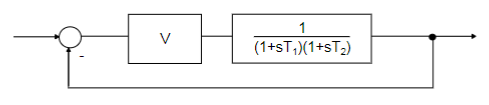
\includegraphics[width=0.6\textwidth]{uebung_5_aufgabe_1.png}
\end{figure}
\begin{paracol}{2}
	\vspace{\fill}
	Übertragungsfunktion aufstellen
	\vspace{\fill}
	\switchcolumn
	\begin{equation*}
		G_0(s) = V \cdot \frac{1}{(1+sT_1)(1+sT_2)}
	\end{equation*}
	\begin{equation}
		G_w(s) = \frac{ V \cdot \frac{1}{(1+sT_1)(1+sT_2)}}{1+(V \cdot \frac{1}{(1+sT_1)(1+sT_2)})}
	\end{equation}
\end{paracol}
\hrule
\begin{paracol}{2}
	\vspace{\fill}
	Gleichung auflösen
	\vspace{\fill}
	\switchcolumn
	\begin{equation}
		lorem\, ipsum
	\end{equation}
\end{paracol}
\hrule
\begin{paracol}{2}
	\vspace{\fill}
	Nenner koeffizienten notieren
	\vspace{\fill}
	\switchcolumn
	\begin{equation*}
		lorem\, ipsum
	\end{equation*}
\end{paracol}
\hrule
\begin{paracol}{2}
	\vspace{\fill}
	Hurwitz-Determinanten aufstellen
	\vspace{\fill}
	\switchcolumn
	\begin{equation*}
		lorem\, ipsum
	\end{equation*}
\end{paracol}


\paragraph{2 Aufgabe:}  Eine nichtschwingungsfähige $IT_2$ -Regelstrecke
\begin{equation*}
	G_S(s) = \frac{k}{(1+sT_1)(1+sT_2)sT_3}
\end{equation*}
soll mit einem Proportionalregler stabilisiert werden.
\begin{enumerate}
	\item Berechnen Sie mit Hilfe des Hurwitz-Kriteriums den allgemeinen Zusammenhang zwischen der kritischen Reglerverstärkung und den Streckenparametern.
	\item Berechnen sie nun die kritische Reglerverstärkung für die Streckenparameter k = 0, 1, $T_1 = 2\, s$, $T_2 = 10\, s$ und $T_3 = 1\, s$.
	\item Zeichnen Sie den Pol-Nullstellenplan des Regelkreises für die Fälle: $V < V_{kr}$, $V = V_{kr}$ und $V > V_{kr}$.
	\item Skizzieren sie den prinzipiellen Verlauf der Übergangsfunktionen des Regelkreises für die genannten Fälle.
\end{enumerate}

\paragraph{3. Aufgabe:} Eine prinzipiell schwingungsfähige IT2 -Regelstrecke \\
\begin{equation*}
	G_S(s) = \frac{k}{(T^2s^2 + 2DT s + 1) T_3s}
\end{equation*}
soll mit einem Proportionalregler stabilisiert werden. \\
Berechnen Sie mit Hilfe des Hurwitz-Kriteriums den allgemeinen Zusammenhang zwischen der kritischen Reglerverst¨arkung und den Streckenparametern.

\paragraph{4. Aufgabe:} Eine prinzipiell schwingungsf¨ahige $PT_2$-Regelstrecke
\begin{equation*}
	GS (s) = \frac{k}{T^2s^2 + 2DTs + 1}
\end{equation*}
soll mit einem Proportionalregler stabilisiert werden. \\
Berechnen Sie mit Hilfe des Hurwitz-Kriteriums den allgemeinen Zusammenhang zwischen der kritischen Reglerverst¨arkung und den Streckenparametern.

\end{document}









